% Figura cuerpo B1: la estrategia de la contraofensiva keynesiana en dos generaciones
\documentclass[tikz,border=3pt]{standalone}
\usepackage[T1]{fontenc}
\usepackage[utf8]{inputenc}
\usetikzlibrary{arrows.meta,calc,positioning}
\begin{document}
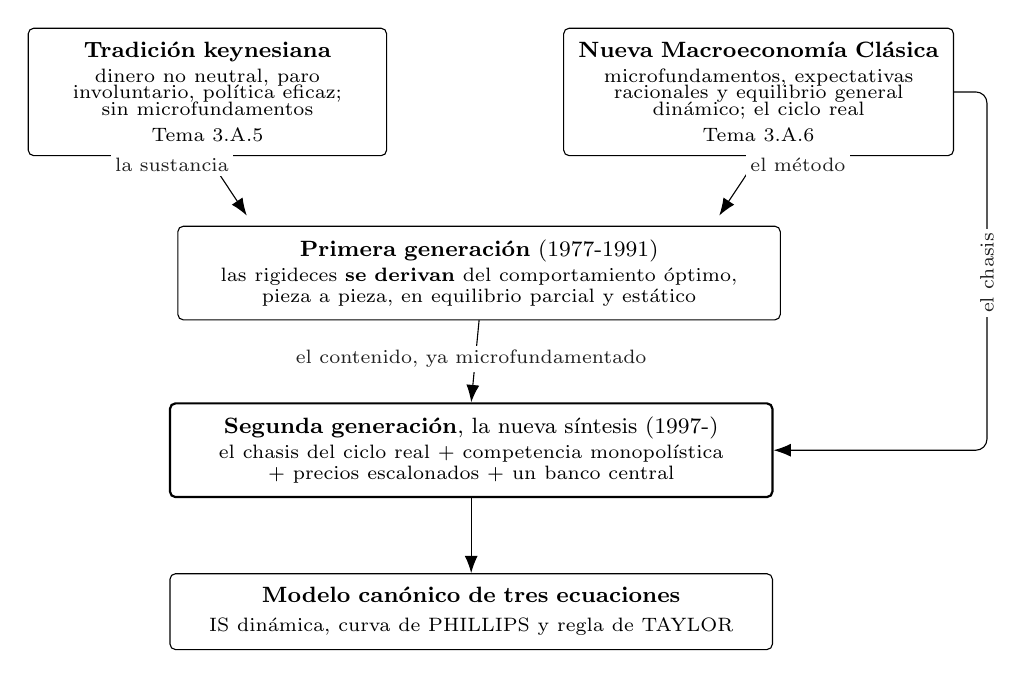
\begin{tikzpicture}[>={Latex[length=2.2mm]}, line cap=round, font=\footnotesize,
  caja/.style={draw, rounded corners=2pt, align=center, inner sep=5pt},
  azul/.style={draw=black, thick, rounded corners=2pt, align=center, inner sep=5pt},
  etq/.style={font=\scriptsize, text=gray!25!black, fill=white, inner sep=1.5pt}]
  % Origenes
  \node[caja, text width=4.2cm] (k) at (2.5,5.25) {\textbf{Tradición keynesiana}\\[1pt]\scriptsize dinero no neutral, paro\\[-2pt]\scriptsize involuntario, política eficaz;\\[-2pt]\scriptsize sin microfundamentos\\\scriptsize Tema 3.A.5};
  \node[caja, text width=4.6cm] (c) at (9.5,5.25) {\textbf{Nueva Macroeconomía Clásica}\\[1pt]\scriptsize microfundamentos, expectativas\\[-2pt]\scriptsize racionales y equilibrio general\\[-2pt]\scriptsize dinámico; el ciclo real\\\scriptsize Tema 3.A.6};
  % Primera generacion
  \node[caja, text width=7.3cm] (n1) at (5.95,2.95) {\textbf{Primera generación} (1977-1991)\\[1pt]\scriptsize las rigideces \textbf{se derivan} del comportamiento óptimo,\\[-2pt]\scriptsize pieza a pieza, en equilibrio parcial y estático};
  \draw[->] (k.south) -- (3.0,3.68);
  \draw[->] (c.south) -- (9.0,3.68);
  \node[etq] at (2.05,4.32) {la sustancia};
  \node[etq] at (10.0,4.32) {el método};
  % Segunda generacion
  \node[azul, text width=7.3cm] (n2) at (5.85,0.70) {\textbf{Segunda generación}, la nueva síntesis (1997-)\\[1pt]\scriptsize el chasis del ciclo real $+$ competencia monopolística\\[-2pt]\scriptsize $+$ precios escalonados $+$ un banco central};
  \draw[->] (n1.south) -- (n2.north);
  \node[etq] at (5.85,1.86) {el contenido, ya microfundamentado};
  \draw[->, rounded corners=4pt] (c.east) -- (12.4,5.25) -- (12.4,0.70) -- (n2.east);
  \node[etq, rotate=90] at (12.4,2.95) {el chasis};
  % Modelo canonico
  \node[caja, text width=7.3cm] (m) at (5.85,-1.35) {\textbf{Modelo canónico de tres ecuaciones}\\[1pt]\scriptsize IS dinámica, curva de PHILLIPS y regla de TAYLOR};
  \draw[->] (n2.south) -- (m.north);
\end{tikzpicture}
\end{document}
